\documentclass{article}
\usepackage[utf8]{inputenc}
\usepackage{amsmath,amssymb}
\usepackage{geometry}
\usepackage{tikz}
\usepackage{chemfig}
\usepackage{chemformula}
\usepackage{enumitem}

\geometry{letterpaper, margin=1in}

\begin{document}

\title{2023 U.S. National Chemistry Olympiad \\ National Exam Part II}
\date{}
\maketitle

\section*{Part II -- Problems \& Explanations}

\subsection*{Question 1 [12\%]}
Compound \ch{A} is an ionic compound that contains only the elements hydrogen, nitrogen, and oxygen.
\begin{enumerate}[label=\alph*.]
    \item A 1.000-g sample of \ch{A} is dissolved in 20 mL water and titrated with 0.5000 M \ch{NaOH} solution, giving the titration curve below. What is the molar mass of \ch{A}?
    
    \begin{center}
    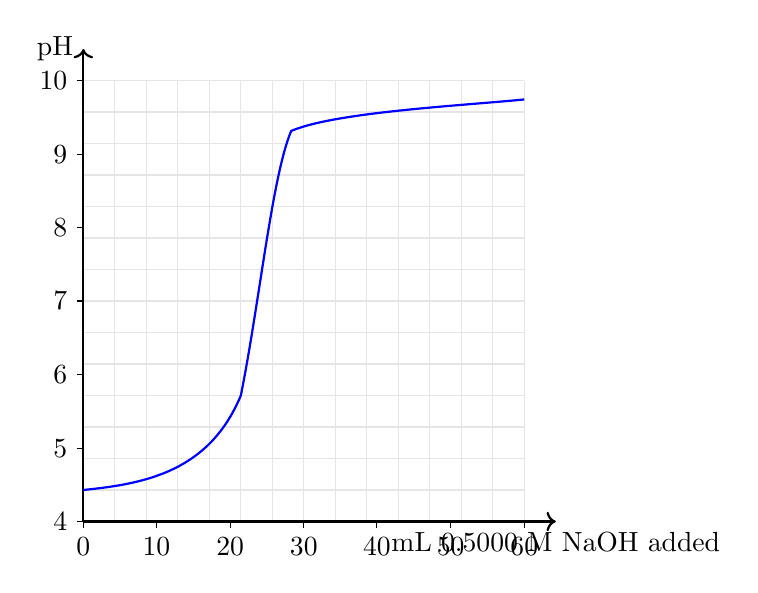
\begin{tikzpicture}[scale=0.8]
        \draw[step=0.5,gray!20,thin] (0,0) grid (7,7);
        \draw[->,thick] (0,0) -- (7.5,0) node[below] {mL 0.5000 M NaOH added};
        \draw[->,thick] (0,0) -- (0,7.5) node[left] {pH};
        \foreach \x/\label in {0/0,1.16/10,2.33/20,3.5/30,4.66/40,5.83/50,7/60}
            \draw (\x,0) -- (\x,-0.1) node[below] {\label};
        \foreach \y/\label in {0/4,1.16/5,2.33/6,3.5/7,4.66/8,5.83/9,7/10}
            \draw (0,\y) -- (-0.1,\y) node[left] {\label};
        \draw[blue,thick] (0,0.5) .. controls (1,0.6) and (2,0.8) .. (2.5,2.0)
                           .. controls (2.8,3.5) and (3.0,5.5) .. (3.3,6.2)
                           .. controls (4,6.5) and (6,6.6) .. (7,6.7);
    \end{tikzpicture}
    \end{center}
    
    \textbf{Answer Space:}
    \vspace{4cm}

    \item When a 1.000-g sample of \ch{A} is heated at 230$^\circ$C in an evacuated 1.50 L vessel, it decomposes into gaseous products, giving a final pressure of 784 mm Hg. How many moles of gas are formed in this reaction?
    
    \textbf{Answer Space:}
    \vspace{4cm}

    \item If the gases produced from the decomposition of 1.000 g of \ch{A} are instead first passed through a column packed with magnesium perchlorate (which strongly absorbs water vapor) and then collected at 25$^\circ$C and a pressure of 755 mm Hg, the total volume of gas is 308 mL. How many moles of gas are collected in this experiment?
    
    \textbf{Answer Space:}
    \vspace{4cm}

    \item What is the formula of \ch{A}? Explain your reasoning.
    
    \textbf{Answer Space:}
    \vspace{5cm}

    \item Write Lewis structures for the cation and the anion present in \ch{A} and for the product(s) of its decomposition at 230$^\circ$C. Your Lewis structures should include all bonds, lone pairs, and nonzero formal charges. Show all significant resonance structures.
    
    \textbf{Answer Space:}
    \vspace{6cm}
\end{enumerate}

\newpage

\subsection*{Question 2 [14\%]}
When water is bound to a metal ion, its acidity increases. For example, the $pK_a$ of \ch{Zn^{2+}(aq)} is 8.96.
\begin{enumerate}[label=\alph*.]
    \item Calculate the pH of a 0.010 M solution of zinc nitrate, \ch{Zn(NO3)2}.
    \vspace{4cm}
    \item Calculate the pH of a 0.010 M solution of zinc acetate, \ch{Zn(CH3COO)2}. The $pK_a$ of \ch{CH3COOH} is 4.75.
    \vspace{4cm}
    \item Zinc hydroxide is sparingly soluble, with $K_{sp} = 4.5 \times 10^{-17}$. Calculate the pH of a solution of water saturated with solid \ch{Zn(OH)2}.
    \vspace{4cm}
    \item Under what circumstances, if any, will a solution of zinc acetate spontaneously form a precipitate of \ch{Zn(OH)2}? If precipitation is possible, specify the circumstances under which it is spontaneous. If it is not possible, justify why not.
    \vspace{4cm}
    \item Zinc also forms a complex ion, \ch{Zn(OH)4^{2-}}, with $K_f = 5.0 \times 10^{14}$. Calculate the solubility of \ch{Zn(OH)2} in a solution with $\text{pH} = 12.00$.
    \vspace{4cm}
\end{enumerate}

\newpage

\subsection*{Question 3 [12\%]}
Hydrogen gas reacts with oxygen gas to give water vapor with $\Delta H^\circ_{rxn} = -241.8\text{ kJ mol}^{-1}$ and $\Delta S^\circ_{rxn} = -44.5\text{ J mol}^{-1}\text{K}^{-1}$:
\[ \ch{H2(g) + 0.5 O2(g) -> H2O(g)} \]
\begin{center}
\begin{tabular}{lcc}
\hline
Species & $S^\circ$, $\text{J mol}^{-1}\text{K}^{-1}$ & $C_p$, $\$text{J g}^{-1}\text{K}^{-1}$ \\ \hline
\ch{H2O(g)} & ??? & 4.18 \\
\ch{H2(g)} & 130.7 & 14.4 \\
\ch{O2(g)} & 205.2 & 0.92 \\ \hline
\end{tabular}
\end{center}
\begin{enumerate}[label=\alph*.]
    \item Calculate $S^\circ$ of \ch{H2O(g)}.
    \vspace{3cm}
    \item The bond dissociation enthalpy (BDE) of an average O-H bond in water is 463 kJ $\text{mol}^{-1}$ and the BDE of the H-H bond in \ch{H2} is 436 kJ $\text{mol}^{-1}$. What is the BDE of the O=O bond in \ch{O2}?
    \vspace{3cm}
    \item 0.100 mol \ch{H2(g)} and 0.100 mol \ch{O2(g)}, both initially at 100$^\circ$C, react completely in a sealed vessel maintained at 1 bar pressure. The vessel is machined as part of a 1.00-kg block of aluminum ($C_p = 0.89\text{ J g}^{-1}\text{K}^{-1}$), which efficiently absorbs the generated heat but is insulated. What is the final temperature?
    \vspace{4cm}
    \item Humid air at 298 K has an overall pressure of 1.0 bar and is 20. vol\% \ch{O2} and 3.1 vol\% \ch{H2O}. What is the minimum volume percentage of \ch{H2(g)} in humid air necessary for its combustion to be spontaneous?
    \vspace{4cm}
    \item Account for the difference between your answer in part d and the experimental value for the lower flammability limit (LFL) of hydrogen gas in humid air ($\approx 4\%$).
    \vspace{3cm}
\end{enumerate}

\newpage

\subsection*{Question 4 [13\%]}
The vapor pressure of pure water at its melting point, 0.0$^\circ$C, is 611 Pa.
\begin{enumerate}[label=\alph*.]
    \item 0.880 mol \ch{MgCl2} is added to 1.00 kg liquid water at 0.0$^\circ$C. Calculate the vapor pressure of this solution.
    \vspace{3.5cm}
    \item The enthalpy of sublimation of ice is 51.1 kJ $\text{mol}^{-1}$ at 0.0$^\circ$C and the enthalpy of vaporization of liquid water is 45.1 kJ $\text{mol}^{-1}$ at 0.0$^\circ$C. Calculate the temperature at which pure ice has the same vapor pressure as the solution at 0.0$^\circ$C.
    \vspace{3.5cm}
    \item At the freezing point temperature of the aqueous magnesium chloride solution, the vapor pressure of the solution is equal to the vapor pressure of pure ice. Explain why this statement is true.
    \vspace{3.5cm}
    \item Using the principle enunciated in part c, calculate the freezing point temperature of the solution.
    \vspace{3.5cm}
    \item As more solid is formed, do you expect the temperature to increase, decrease, or remain constant? Briefly justify.
    \vspace{3.5cm}
\end{enumerate}

\newpage

\subsection*{Question 5 [12\%]}
Write net equations for each of the reactions below.
\begin{enumerate}[label=\alph*.]
    \item Aqueous hydrochloric acid is added to a solution of sodium hypochlorite.
    \vspace{2cm}
    \item Aluminum foil is added to concentrated aqueous potassium hydroxide solution.
    \vspace{2cm}
    \item Metallic sodium is added to liquid ammonia in the presence of a trace amount of iron(III) nitrate.
    \vspace{2cm}
    \item Potassium tetrachloroplatinate is heated with two equivalents of aqueous ammonia.
    \vspace{2cm}
    \item Sodium tert-butoxide is added to 3-bromo-3-ethylpentane in DMF solution.
    \vspace{2cm}
    \item Cobalt-57 undergoes radioactive decay by electron capture.
    \vspace{2cm}
\end{enumerate}

\newpage

\subsection*{Question 6 [12\%]}
The standard reduction potentials of some compounds of platinum and silver at 298 K are given below:
\begin{center}
\begin{tabular}{lc}
\hline
Half-reaction & $E^\circ$, V \\ \hline
\ch{Pt^{2+}(aq) + 2e^- -> Pt(s)} & +1.188 \\
\ch{PtCl4^{2-}(aq) + 2e^- -> Pt(s) + 4Cl^-(aq)} & +0.758 \\
\ch{PtCl6^{2-}(aq) + 2e^- -> PtCl4^{2-}(aq) + 2Cl^-(aq)} & +0.726 \\
\ch{Ag^+(aq) + e^- -> Ag(s)} & +0.799 \\ \hline
\end{tabular}
\end{center}
\begin{enumerate}[label=\alph*.]
    \item What is $K_f$ for the \ch{PtCl4^{2-}} ion?
    \vspace{3.5cm}
    \item What is $E^\circ$ for the reduction of hexachloroplatinate(IV) to give platinum metal?
    \vspace{3.5cm}
    \item What is the minimum potential that would need to be applied to the electrolytic cell shown below in order to cause the platinum electrode to dissolve to form \ch{PtCl4^{2-}(aq)} and the \ch{Ag^+(aq)} to deposit on the Ag electrode?
    \vspace{3.5cm}
    \item As electrolysis is carried out, is it thermodynamically possible for a significant amount of hexachloroplatinate(IV) to be produced at the anode? Justify your answer.
    \vspace{3.5cm}
\end{enumerate}

\newpage

\subsection*{Question 7 [13\%]}
\begin{enumerate}[label=\alph*.]
    \item Draw or clearly describe the shapes of the molecules \ch{BF3} and \ch{NF3}.
    \vspace{2.5cm}
    \item In all cases, the normal boiling points of the \ch{AF_n} molecules are lower than those of the \ch{A(CH3)_n} molecules. Explain this observation.
    \vspace{2.5cm}
    \item Not counting the boron compounds, the trend in boiling points is that they decrease as the central atom A moves to the right in the periodic table. Explain this trend.
    \vspace{2.5cm}
    \item Explain why \ch{BF3} has a higher boiling point than \ch{CF4}, while \ch{B(CH3)3} has a lower boiling point than \ch{C(CH3)4}.
    \vspace{2.5cm}
    \item Explain why the A-C bond distances decrease as A moves to the right in the periodic table.
    \vspace{2.5cm}
    \item Explain why the A-F bond distances increase as A moves to the right in the periodic table.
    \vspace{2.5cm}
\end{enumerate}

\newpage

\subsection*{Question 8 [12\%]}
Consider cyclopentanone and 1-methylcyclopentene.
\begin{enumerate}[label=\alph*.]
    \item Which compound has the higher normal boiling point? Justify your choice.
    \vspace{3cm}
    \item One of the two compounds will rapidly decolorize bromine in carbon tetrachloride. Which one? Draw the structure of the major product, showing stereochemistry.
    \vspace{3cm}
    \item One of the two compounds will react rapidly with methylmagnesium bromide. Which one? Draw the structure of the major organic product after workup.
    \vspace{3.3cm}
    \item Specify how the product of part c can be transformed into either cyclopentanone or 1-methylcyclopentene in a single reaction.
    \vspace{3cm}
    \item Draw the structure of an acyclic isomer of 1-methylcyclopentene that is chiral.
    \vspace{3cm}
\end{enumerate}


\newpage
\section*{Solutions \& Answer Key}

\subsection*{Question 1 Solutions}
\begin{enumerate}[label=\alph*.]
    \item Molar mass calculation: Endpoint is at 25.0 mL.
    \[ n = (0.0250\text{ L})(0.5000\text{ M}) = 0.0125\text{ mol} \]
    \[ \text{Molar mass} = \frac{1.000\text{ g}}{0.0125\text{ mol}} = 80.0\text{ g mol}^{-1} \]
    \item Moles of gas: $PV = nRT \implies n = \frac{(784/760\text{ atm})(1.50\text{ L})}{(0.08206\text{ L atm mol}^{-1}\text{K}^{-1})(503.15\text{ K})} = 0.0375\text{ mol}$.
    \item Moles of dry gas: $PV = nRT \implies n = \frac{(755/760)(0.308)}{(0.08206)(298.15)} = 0.0125\text{ mol}$.
    \item Formula: \ch{(NH4)NO3} (Ammonium nitrate).
    \item Lewis Structures:
    \begin{center}
        \textbf{Cation:} [\ch{NH4+}] \quad
        \textbf{Anion (Resonance):} \\
        \chemfig{N([:90]=O)([:-30]-O^{-})([:-150]-O^{-})} \quad $\longleftrightarrow$ \quad \chemfig{N([:90]-O^{-})([:-30]=O)([:-150]-O^{-})}
    \end{center}
\end{enumerate}

\subsection*{Question 2 Solutions}
\begin{enumerate}[label=\alph*.]
    \item $\text{pH} = 5.48$
    \item $\text{pH} = 7.01$
    \item $\text{pH} = 8.65$
    \item Spontaneous if $[\ch{Zn^{2+}}] > 4.3 \times 10^{-3}\text{ M}$.
    \item Solubility $= 2.3 \times 10^{-6}\text{ M}$.
\end{enumerate}

\subsection*{Question 3 Solutions}
\begin{enumerate}[label=\alph*.]
    \item $S^\circ(\ch{H2O(g)}) = 188.8\text{ J mol}^{-1}\text{K}^{-1}$
    \item $\text{BDE}(\ch{O=O}) = 496\text{ kJ mol}^{-1}$
    \item $T_f = 400\text{ K } (127^\circ\text{C})$
    \item Minimum vol\% of \ch{H2} $= 6.1 \times 10^{-40}\%$.
    \item Flammability limit is determined by kinetics, not thermodynamics.
\end{enumerate}

\subsection*{Question 4 Solutions}
\begin{enumerate}[label=\alph*.]
    \item $P = 584\text{ Pa}$
    \item $T = 272.6\text{ K } (-0.5^\circ\text{C})$
    \item At equilibrium, chemical potentials of water in both phases must be equal.
    \item $T_f = 268.5\text{ K } (-4.7^\circ\text{C})$
    \item Temperature decreases as the remaining solution becomes more concentrated.
\end{enumerate}

\subsection*{Question 5 Solutions}
\begin{enumerate}[label=\alph*.]
    \item \ch{H^+ + Cl^- + OCl^- -> Cl2 + H2O}
    \item \ch{Al + OH^- + H2O -> Al(OH)4^- + H2}
    \item \ch{Na + NH3 -> Na^+ + NH2^- + H2}
    \item Tetrachloroplatinate with ammonia: \\
    \chemfig{Pt([:45]-Cl)([:135]-Cl)([:-135]-NH_3)([:-45]-NH_3)}
    \item Elimination reaction product: \\
    \chemfig{C(=[4]C)(-[2]CH_3)(-[6]CH_2CH_3)}
    \item \ch{^{57}_{27}Co + e^- -> ^{57}_{26}Fe + \gamma}
\end{enumerate}

\subsection*{Question 6 Solutions}
\begin{enumerate}[label=\alph*.]
    \item $K_f = 3.5 \times 10^{14}$
    \item $E^\circ = +0.742\text{ V}$
    \item $E = -0.048\text{ V}$
    \item Yes, because the standard potential for the oxidation is thermodynamically competitive.
\end{enumerate}

\subsection*{Question 7 Solutions}
\begin{enumerate}[label=\alph*.]
    \item \ch{BF3} is trigonal planar; \ch{NF3} is trigonal pyramidal.
    \item F has lower polarizability due to high electronegativity, reducing London dispersion forces.
    \item Decreasing number of electrons reduces dispersion forces.
    \item \ch{BF3} has intermolecular Lewis acid-base interactions.
    \item Increasing effective nuclear charge contracts the atomic radius.
    \item Lone pair-lone pair repulsions increase as central atom moves right.
\end{enumerate}

\subsection*{Question 8 Solutions}
\begin{enumerate}[label=\alph*.]
    \item Cyclopentanone due to strong dipole-dipole interactions of the \ch{C=O} bond.
    \item 1-methylcyclopentene. Product: \\
    \chemfig{[:18]*5(--(-Br)-(-Br?)(~[2]CH_3)--)}
    \item Cyclopentanone. Product after workup: 1-methylcyclopentanol \\
    \chemfig{[:18]*5(--(-OH)(~[2]CH_3)---)}
    \item Acid-catalyzed dehydration using \ch{H2SO4} and heat converts it to 1-methylcyclopentene.
    \item Chiral acyclic isomer: \\
    \chemfig{C([4]-H)([2]-CH_3)([-2]-CH_2CH_3)(-[0]C\#CH)}
\end{enumerate}

\end{document}